\documentclass{beamer}
\usefonttheme{professionalfonts}
\usepackage[english]{babel}
\usepackage{geometry}
\usepackage{amsmath}
\usepackage{amsthm}
\usepackage{graphicx}
\usepackage{caption}
\usepackage[utf8]{inputenc}

%%%%%%%% HYPERREF PACKAGE
\hypersetup{colorlinks=true}
\hypersetup{citecolor=orange}
\hypersetup{urlcolor=orange}

%%%%%%%% DEFINITION AND THEOREM DEFINITIONS
\let\definition\relax
\theoremstyle{definition}
\newtheorem{definition}{Definition}[section]

\let\remark\relax
\theoremstyle{remark}
\newtheorem{remark}{Remark}

\theoremstyle{example}
\newtheorem{question}{Question}

%%%%%%%% MULTI-COLUMNS PACKAGE
\usepackage{multicol}

%%%%%%%% BIB-LATEX STUFF
\usepackage[style=authoryear,
            bibstyle=authoryear,
            citestyle=authoryear,
            hyperref=true,
            backend=biber]{biblatex}
\addbibresource{ref.bib} % Bibliography file

%%%%%%%% ICONS FOR CITES
% https://tex.stackexchange.com/questions/68080/beamer-bibliography-icon
\setbeamertemplate{bibliography item}{%
  \ifboolexpr{ test {\ifentrytype{book}} or test {\ifentrytype{mvbook}}
    or test {\ifentrytype{collection}} or test {\ifentrytype{mvcollection}}
    or test {\ifentrytype{reference}} or test {\ifentrytype{mvreference}} }
    {\setbeamertemplate{bibliography item}[book]}
    {\ifentrytype{online}
       {\setbeamertemplate{bibliography item}[online]}
       {\setbeamertemplate{bibliography item}[article]}}
  \usebeamertemplate{bibliography item}}

\defbibenvironment{bibliography}
  {\list{}
     {\settowidth{\labelwidth}{\usebeamertemplate{bibliography item}}
      \setlength{\leftmargin}{\labelwidth}
      \setlength{\labelsep}{\biblabelsep}
      \addtolength{\leftmargin}{\labelsep}
      \setlength{\itemsep}{\bibitemsep}
      \setlength{\parsep}{\bibparsep}}}
  {\endlist}
  {\item}

%%%%%%%% BRACKETS AROUND CITE
% https://tex.stackexchange.com/questions/16765/biblatex-author-year-square-brackets
\makeatletter

\newrobustcmd*{\parentexttrack}[1]{
  \begingroup
  \blx@blxinit
  \blx@setsfcodes
  \blx@bibopenparen#1\blx@bibcloseparen
  \endgroup}

\AtEveryCite{
  \let\parentext=\parentexttrack
  \let\bibopenparen=\bibopenbracket
  \let\bibcloseparen=\bibclosebracket}

\makeatother

%%%%%%%% THEME SLIDES
\usetheme{default}

%%%%%%%% BEAMER STUFF
\setbeamertemplate{footline}[frame number]
\setbeamertemplate{section in toc}[sections numbered]
\setbeamertemplate{subsection in toc}[subsections numbered]
\setbeamertemplate{navigation symbols}{}

% Not enumerate frame breaks
% https://tex.stackexchange.com/questions/295854/how-to-edit-behaviour-of-frame-titles-during-frame-break-in-beamer
\setbeamertemplate{frametitle continuation}[from second][]

%%%%%%%% FRAME TITLES AND SUBTITLES
% https://stackoverflow.com/questions/35810906/vim-beamer-dynamic-frame-title1
\newif\ifinsection
\newif\ifinsubsection

\let\oldsection\section
\renewcommand{\section}{
  \global\insectiontrue
  \global\insubsectionfalse
  \oldsection}
\let\oldsubsection\subsection
\renewcommand{\subsection}{
  \global\insubsectiontrue
  \oldsubsection}

\newcommand {\aframe}[1] {
  \begin{frame}
    \ifinsection\frametitle{\secname}\fi
    \ifinsubsection\framesubtitle{\subsecname}\fi
  #1
  \end{frame}
}

% Blue line after title
% https://tex.stackexchange.com/questions/343517/beamer-full-width-hrule-below-frame-title
\setbeamertemplate{frametitle}{%
    \usebeamerfont{frametitle}\insertframetitle\strut%
    \vskip.0\baselineskip%
    \leaders\vrule width 0.85\paperwidth\vskip0.4pt%
    \vskip2pt%
    \usebeamerfont{framesubtitle}\insertframesubtitle
}

%%%%%%%% FOOTNOTE STUFF
\renewcommand{\thefootnote}{\fnsymbol{footnote}}
% Footnote without symbol
% https://tex.stackexchange.com/questions/30720/footnote-without-a-marker
\newcommand\blfootnote[1]{%
  \begingroup
  \renewcommand\thefootnote{}\footnote{#1}%
  \addtocounter{footnote}{-1}%
  \endgroup
}

%%%%%%%% CENTER OF SLIDE THANK YOU
\usepackage{tikz}

%%%%%%%% SUB-FIGURE PACKAGE
\usepackage{subcaption}

%%%%%%%% PERSONAL COMMANDS
\usepackage{amssymb}

%%%% Important sets
\renewcommand{\O}{\mathbb{O}}
\newcommand{\N}{\mathbb{N}}
\newcommand{\Z}{{\mathbb{Z}}}
\newcommand{\Q}{{\mathbb{Q}}}
\newcommand{\R}{{\mathbb{R}}}

%%%% Usual operations
\newcommand{\pow}[2]{#1^{#2}}
\newcommand{\expp}[1]{e^{#1}}
\newcommand{\fst}{\mathrm{fst} \,}
\newcommand{\snd}{\mathrm{snd} \,}

%%%% Lambda Calculus Symbols
\newcommand{\dneq}{\,\, \# \,\,}
\renewcommand{\S}{\pmb{\mathrm{S}}}
\newcommand{\I}{\pmb{\mathrm{I}}}
\newcommand{\K}{\pmb{\mathrm{K}}}
\newcommand{\ch}[1]{\ulcorner #1 \urcorner}

%%%% Ordinal Lambda Calculus Symbols
\newcommand{\ordAlph}{\Sigma_{\text{Ord}}}
\newcommand{\termOrd}{\text{Term}_\text{Ord}}
\newcommand{\fl}{\mathrm{fl}}
\newcommand{\sk}{\mathrm{sk}}

%%%% Superscript to the left
% https://latex.org/forum/viewtopic.php?t=455
\usepackage{tensor}
\newcommand{\app}[3]{\tensor*[^{#1}]{\left(#2, #3\right)}{}}

%%%% Make optional parameter
% https://tex.stackexchange.com/questions/217757/special-behavior-if-optional-argument-is-not-passed
\usepackage{xparse}

%%%% Statistics
\NewDocumentCommand{\E}{o m}{
  \IfNoValueTF{#1}
  {\mathbb{E}\left[#2\right]}
  {\mathbb{E}^{#1}\left[ #2\right]}
}
\NewDocumentCommand{\V}{o m}{
  \IfNoValueTF{#1}
  {\mathrm{Var}\left[#2\right]}
  {\mathrm{Var}^{#1}\left[ #2\right]}
}
\RenewDocumentCommand{\P}{o m}{
  \IfNoValueTF{#1}
  {\mathrm{P}\left[#2\right]}
  {\mathrm{P}^{#1}\left[ #2\right]}
}

%%%% Lambda Calculus
\NewDocumentCommand{\cx}{o}{
  \IfNoValueTF{#1}
  {\left[\quad\right]}
  {\left[\, #1 \,\right]}
}

%%%%%%%% LOGIC TREES
\usepackage{prftree}

%%%%%%%% SPLIT EQUATIONS
% https://tex.stackexchange.com/questions/51682/is-it-possible-to-pagebreak-aligned-equations
\allowdisplaybreaks

%%%%%%%% TO USE SHORT COMMANDS FOR VECTOR LINES
\usepackage{esvect}

%%%%%%%% START DOCUMENT
\title{Exercise 3.5.7}

\author{Juan Sebasti\'an C\'ardenas-Rodríguez \\
  \scalebox{0.7}{Mathematical Engineering, Universidad EAFIT}}

\begin{document}

% Plain so is not numbered
\begin{frame}[plain]
  \titlepage
\end{frame}

%%%%%%%%%% SLIDES %%%%%%%%%%%%%%%
\section{Exercise \textit{i)}}
\subsection{Problem Statement}
\aframe{ Show that if $G_1$ and $G_2$ are the $\beta$-graphs of some
  term, then so is their cartesian product. \pause

  \begin{definition}
    Let $V_1$, $V_2$ be the set of vertices, of graphs $G_1$ and $G_2$
    respectively. Let $E_1$, $E_2$ be the set of edges of those same graphs.
    Then,\textcite{harary1969} defines the graph $G_1 \times G_2$ as:
    \begin{itemize}
      \item Set of vertices $V = V_1 \times V_2$ \pause
      \item Set of edges:
            \begin{equation*}
              E = \{(u, v) \in V \times V \mid \mathrm{prop1} \, u \, v \vee
              \mathrm{prop2} \, u \, v\}
            \end{equation*}
            where
            \begin{align*}
              \mathrm{prop1} \, u \, v
              &:= (\fst u = \fst v \wedge (\snd u, \snd v) \in E_2) \\
              \mathrm{prop2} \, u \, v
              &:= (\snd u = \snd v \wedge (\fst u, \fst v) \in E_1)
            \end{align*}
    \end{itemize}
  \end{definition}
}

\subsection{Solution Vertices}
\aframe{Let's see that if $G_1$ and $G_2$ are the reduction graphs of
  terms $M$ and $N$ respectively then the graph $G_1 \times G_2$ is
  the reduction graph of $MN$. \pause
  \begin{proof}
    In first place, let's find a function that transforms tuples of
    $\lambda$-terms to a term. Hence, let $f$ be that function such
    that:
    \begin{equation*}
      f((u_1, u_2)) = u_1u_2
    \end{equation*}
    \pause \textbf{Why is $u_1u_2$ a vertex?} \pause
    \begin{alignat*}{2}
      M &\twoheadrightarrow_\beta u_1  \quad &&N \twoheadrightarrow_\beta u_2 \\
      MN &\twoheadrightarrow_\beta u_1N \quad &&u_1N \twoheadrightarrow_\beta u_1u_2 \\
      &\quad MN \twoheadrightarrow_\beta &&u_1u_2
    \end{alignat*}
  \end{proof}
}

\section{Exercise \textit{ii)}}
\subsection{Problem Statement}
\aframe{ If $G$ is the $\beta$-graph of a term, then $G \mapsto K_1$
  (add one point that is below each point of $G$). \pause
  \begin{figure}[t]
    \centering
    \begin{subfigure}[b]{0.45\textwidth}
      \centering
      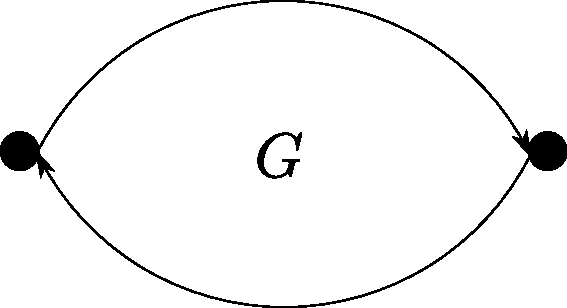
\includegraphics[scale=0.35]{../../graphs/exercise-3-5-7-ii-example-G}
      \caption{$G$ graph.}
    \end{subfigure} \pause
    \begin{subfigure}[b]{0.45\textwidth}
      \centering
      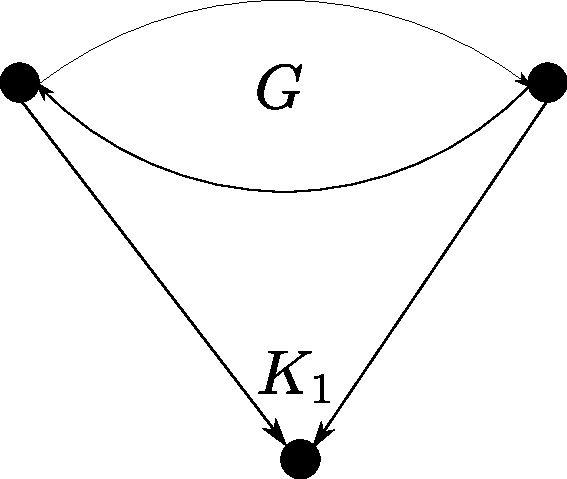
\includegraphics[scale=0.35]{../../graphs/exercise-3-5-7-ii-example-G-with-K}
      \caption{$G \mapsto K_1$ graph.}
    \end{subfigure} \pause
  \end{figure}
  Hence, the set of edges and vertices would be of the form:
    \begin{align*}
      V &= \{v | v \text{ is a vertex of } G\} \cup \{K_1\} \\
      E &= \{(u, v) \mid (u, v) \text{ is a edge of } G\} \cup
          \{(u, K_1) \mid u \text{ is a vertex of } G\}
    \end{align*}
  }

\subsection{Solution}
\aframe{ Intuitively, if $G$ is the graph of a term $M$ then the term
  of the graph $G \mapsto K_1$ must be $\K^* M$. \pause \\
  \vspace{0.5cm}

  \begin{proof}
    It is clear that for all $N$ such that
    $M \twoheadrightarrow_\beta N$, then it happens that:
    \begin{equation*}
      \K^* M \twoheadrightarrow_\beta \K^* N
    \end{equation*} \pause
    Hence the vertices and edges of the reduction graph of the term $\K^* M$
    are given by:
  \begin{align*}
    \onslide{V =& \{\K^*N \mid M \twoheadrightarrow_\beta N \} \cup \{\I\} \\}
    \onslide<4->{E = &\{(\K^*N, \K^*L) \mid N \rightarrow_\beta L
          \wedge N, L \text{ are vertices of } G \} \cup \\
      &\{(N, \I) \mid N \text{ is a vertex of } G\}}
  \end{align*}
  \end{proof}
}

%%%%%%%%%%%%%%%%%%%%%%%%%%%%%%%%%
\begin{frame}[allowframebreaks]{References}
  \printbibliography
\end{frame}

\begin{frame}
  \begin{tikzpicture}[overlay, remember picture]
     \node[anchor=center] at (current page.center) {
     \Huge{\emph{Thank you!}}};
\end{tikzpicture}
  \begin{minipage}[t][.8\textheight]{\textwidth}
    \vfill
    \begin{center}
        \scalebox{0.7}{Juan Sebasti\'an C\'ardenas-Rodríguez} \\
        \scalebox{0.7}{jscardenar@eafit.edu.co} \\
    \end{center}
  \end{minipage}
\end{frame}

\end{document}
